\chapter{Dataset}
All the experimental work was carried out on the Kvasir Capsule Endoscopy Dataset\cite{data}. 
\section{Data set}
A segment of Kvasir-Capsule, a video capsule endoscopy data set, is used for this project.
Each image has 336x336 dimensions and is in RGB colour code. There are total of 47236 images belonging to different sub-categories of medical anomalies.
The original dataset had the images as shown in Table \ref{Table:4.1}
\begin{table}[h!]
\centering
\caption{Table of original data set.}
\begin{tabular}{ |c|c| }
\hline
 Normal clean mucosa & 34338 \\
 Ileocecal valve & 4189 \\
 Reduced mucosal view & 2096 \\
 Pylorus    &    1529 \\
 Angiectasia         &     866 \\
 ulcer               &     854 \\
 Foreign body        &     766\\    
 Lymphangiectasia    &     592 \\
 Erosion             &     506 \\
 Blood - fresh       &     446 \\
 Erythema            &      159 \\
 Polyp               &      55 \\
 Blood - hematin     &       12 \\
 ampulla of water    &        10 \\
\hline
\end{tabular}
\label{Table:4.1}
\end{table}
\newline
The Experimentation was carried on multiple subsets of the original Dataset.
Initially 10,000 training images were randomly sampled from the original set with 1000 testing images. Few sample images from the dataset are given in Fig.\ref{fig:label4.1}
\begin{figure}[h]
    \centering
    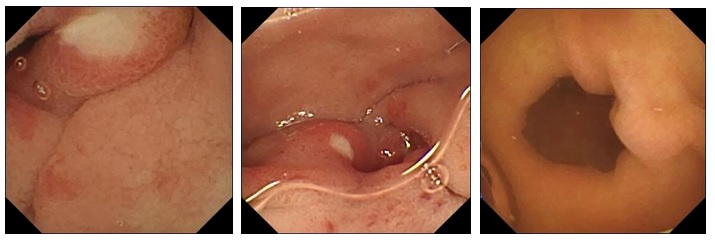
\includegraphics[totalheight=1.5in]{Chapter4/Fig4.1.jpg}
    \caption[Glimpse of uncropped capsule images]{Glimpse of uncropped capsule images.\cite{data}}
    \label{fig:label4.1}
\end{figure}
\newpage
As we can see in the sample images Fig.\ref{fig:label4.1} that the corner of the images are complete black spaces, while feeding this data to the image super resolution network for learning purposes, the network was not able to learn well and an semi transparent white layer was observed on the output images. To overcome this problem, we feed the network with cropped images, that didn't have any blank spot in the corners.
The glimpse of that dataset is shown in Fig.\ref{fig:label4.2}
\begin{figure}[h]
    \centering
    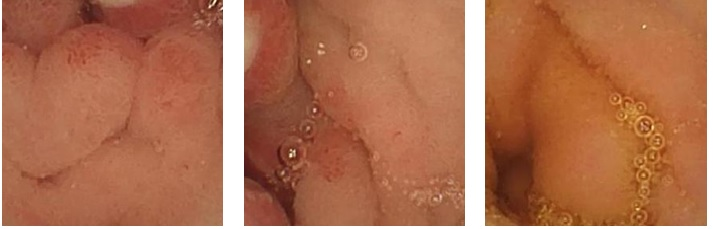
\includegraphics[totalheight=1.5in]{Chapter4/Fig4.2.jpg}
    \caption[Glimpse of Cropped dataset]{Glimpse of Cropped dataset.\cite{data}}
    \label{fig:label4.2}
\end{figure}
\newline
As Image super resolution is a comperatively complex task, the network was not able to perform well when the input data belonged to multiple classes, as the underlying spartial information was different for different classes. Hence a new dataset was developed which was the subset of original dataset of cropped images.
The final training of all the models/networks was done on this dataset. After cropping, the resolution of the cropped images is $228 \times 228$ pixels, which was $336 \times 336$ pixels originally.